\section{Funktionsweise}

\begin{frame}{Begriffe}
  \begin{Definition}
    Ein \textbf{Repository} ist ein verwaltetes Verzeichnis zur Speicherung und Beschreibung von digitalen Objekten für ein digitales Archiv.\cite{WREP}
  \end{Definition}

  \begin{Definition}
    \textbf{Remote origin} ist ein Verweis auf das \textit{remote} Repository (also eine URL).
  \end{Definition}
\end{frame}

\begin{frame}[fragile]{.git Ordner}
  \begin{itemize}
    \item Alle \textbf{git-Daten} liegen im .git Repository mit optionalen Ausnahmen
  \end{itemize}
  \pause
  \begin{lstlisting}[basicstyle=\tiny]
  $ ls -l .git
  total 40
  -rw-r--r--   1 joeldierkes  staff   15 Mar 29 21:43 COMMIT_EDITMSG
  -rw-r--r--   1 joeldierkes  staff   23 Mar 29 21:43 HEAD
  -rw-r--r--   1 joeldierkes  staff  137 Mar 29 21:43 config
  -rw-r--r--   1 joeldierkes  staff   73 Mar 29 21:43 description
  drwxr-xr-x  13 joeldierkes  staff  416 Mar 29 21:43 hooks
  -rw-r--r--   1 joeldierkes  staff  209 Mar 29 21:43 index
  drwxr-xr-x   3 joeldierkes  staff   96 Mar 29 21:43 info
  drwxr-xr-x   4 joeldierkes  staff  128 Mar 29 21:43 logs
  drwxr-xr-x  10 joeldierkes  staff  320 Mar 29 21:43 objects
  drwxr-xr-x   4 joeldierkes  staff  128 Mar 29 21:43 refs
  \end{lstlisting}
\end{frame}

\begin{frame}{Blob}
  \begin{Definition}
    Ein \textbf{Blob} (\glqq \textit{binary large object} \grqq ) ist eine Version einer Datei.
  \end{Definition}
  \begin{itemize}
    \pause
    \item Enthält den Inhalt einer Datei, aber nicht deren Metadaten (Dateiname, Erstelldatum, ...)
    \pause
    \item Ist eindeutig durch den SHA-1 Wert bestimmt (Kollision verschwindend gering)
  \end{itemize}
\end{frame}

\begin{frame}{Tree}
  \begin{Definition}
    Ein \textbf{Tree} enthält Informationen eines Systemordners.
  \end{Definition}
  \begin{itemize}
    \pause
    \item Verweist auf Blobs und weitere (Sub-)Trees.
    \pause
    \item Enthält ebenfalls keine Meta Daten
    \pause
    \item Ist ebenfalls eindeutig durch den SHA-1 Wert bestimmt
  \end{itemize}
\end{frame}

\begin{frame}{Commit}
  \begin{Definition}
    Ein \textbf{Commit} enthält Informationen zu einer Änderung des Repositories.
  \end{Definition}
  \begin{itemize}
    \pause
    \item Verweist auf einen Tree, einen oder mehrere \glqq Parent\grqq{} Commits, einen Autor, ein Datum und weitere Informationen
    \pause
    \item Hat einen semantischen Sinnzusamenhang
    \pause
    \item Ist ebenfalls eindeutig durch den SHA-1 Wert bestimmt
  \end{itemize}
\end{frame}

\begin{frame}{Commit}
  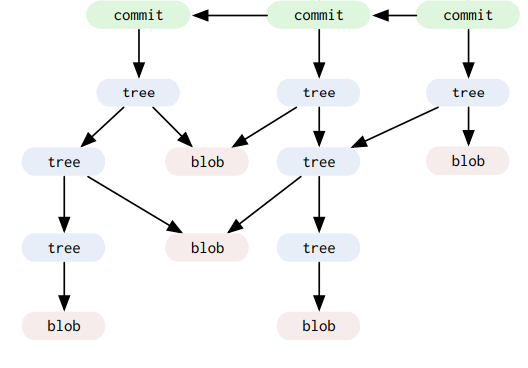
\includegraphics[scale=0.5]{./section/pictures/internes.png}
\end{frame}

\begin{frame}{Tags}
  \begin{Definition}
    Ein \textbf{Tag} referenziert auf ein Objekt, meistens ein Commit.
  \end{Definition}
  \begin{itemize}
    \pause
    \item Sollte einen sinnvollen Namen besitzen
  \end{itemize}
\end{frame}

\begin{frame}{Index}
  \begin{itemize}
    \item Referenziert die Blobs und Trees auf Systemdateien/-ordner
  \end{itemize}
\end{frame}
